
\chapter{Конструкторская часть}\label{Konstruct}
%\addcontentsline{toc}{chapter}{2 Конструкторская часть}

\section{Схемы алгоритмов}\label{SchemaAlg}


\subsection{Схема матричного алгоритма поиска расстояния Левенштейна}\label{SchemaMatrixLeventshein}

На рисунке \ref{ris:levenshteinmatrixschema} показана схема алгоритма расчета расстояния Левенштейна матричным способом.

\begin{figure}[H]
  \center{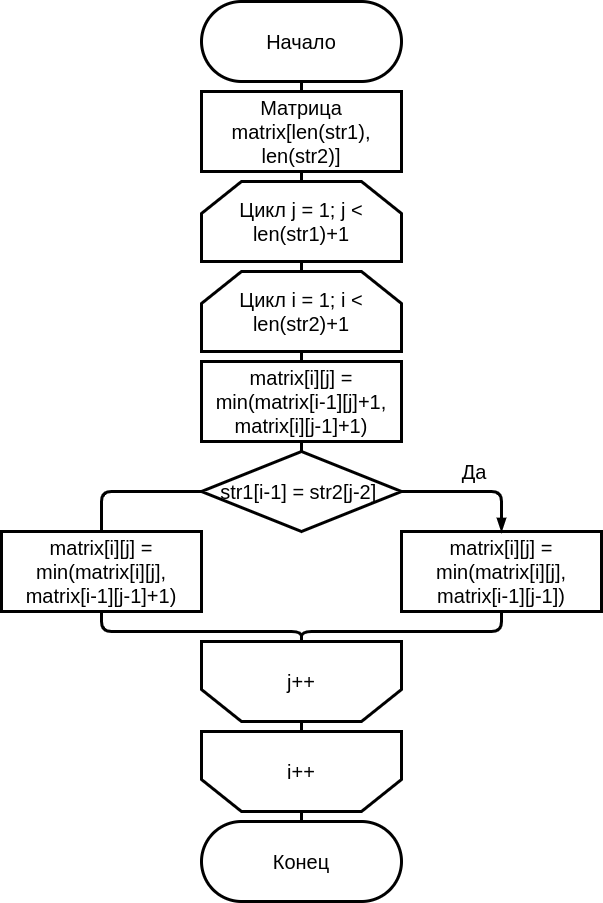
\includegraphics[scale=0.35]{l1.levenshteinmatrixschema}}
  \caption{Схема алгоритма нахождения расстояния Левенштейна матричным способом}
  \label{ris:levenshteinmatrixschema}
\end{figure}



\subsection{Схема рекурсивного алгоритма поиска расстояния Левенштейна}\label{SchemaRecursLeventshein}

На рисунке \ref{ris:levenshteinrecursiveschema} показана схема алгоритма расчета расстояния Левенштейна с помощью рекурсии.

\begin{figure}[H]
    \center{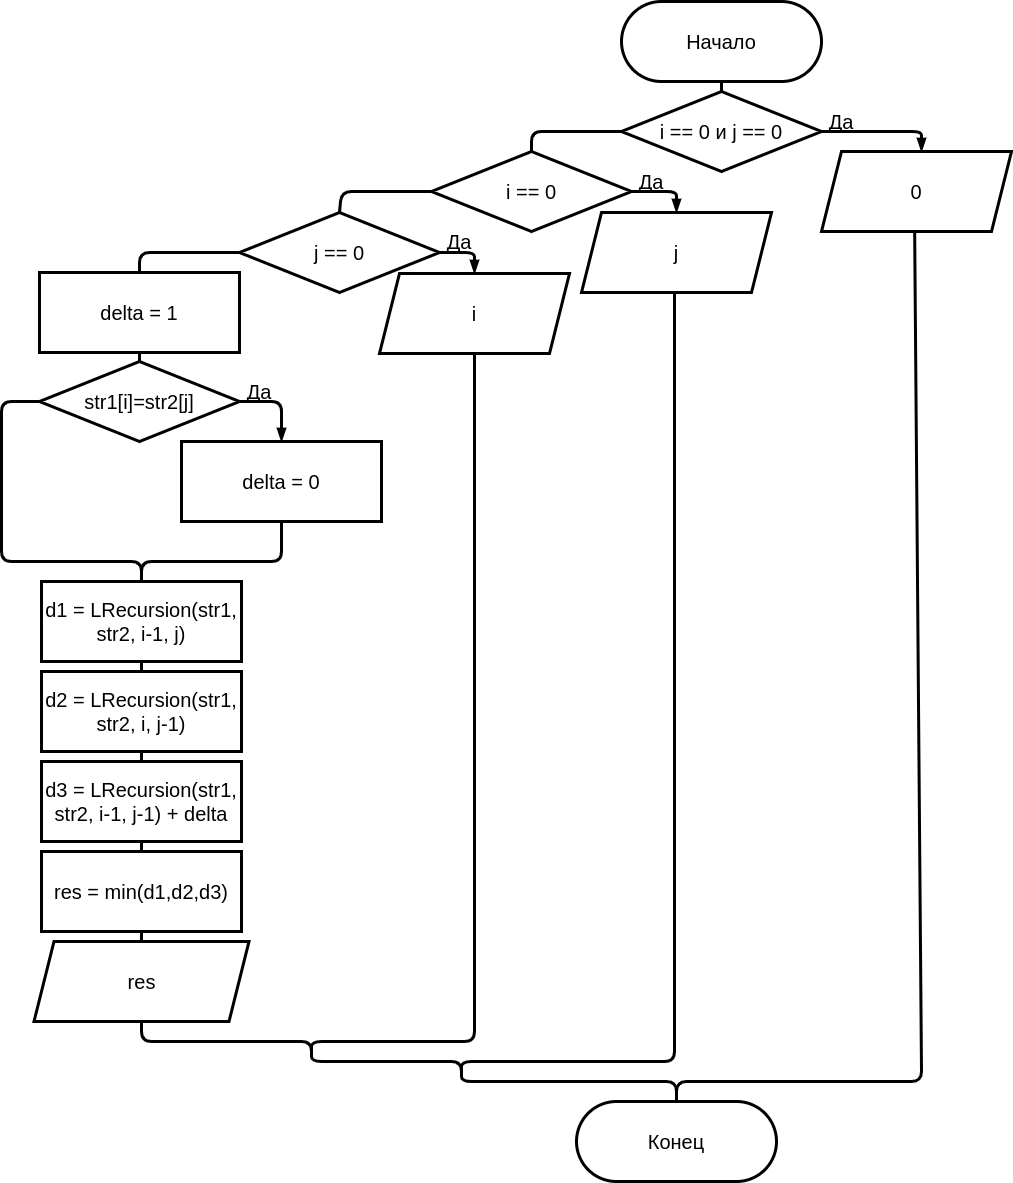
\includegraphics[scale=0.35]{l1.levenshteinrecursiveschema}}
    \caption{Схема алгоритма нахождения расстояния Левенштейна рекурсивным способом}
    \label{ris:levenshteinrecursiveschema}
\end{figure}

\subsection{Схема рекурсивного алгоритма поиска расстояния Левенштейна с кешем}\label{SchemaRecursKeshLeventshein}

На рисунке \ref{ris:levenshteinrecursivekeshschema} показана схема алгоритма расчета расстояния Левенштейна с помощью рекурсии с кешем.

\begin{figure}[H]
    \center{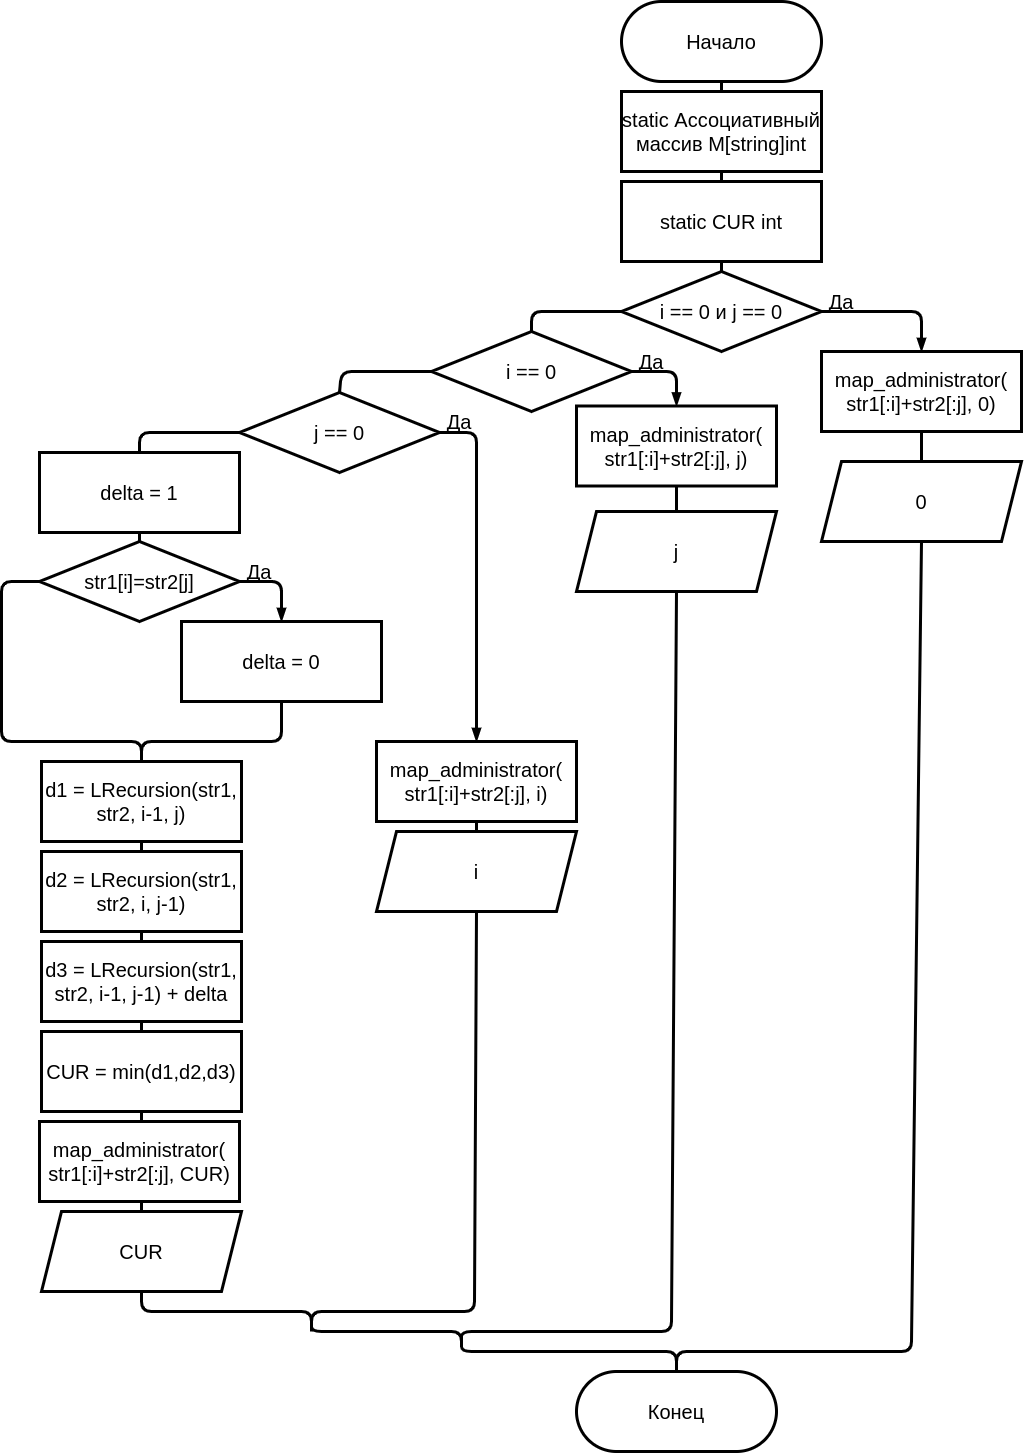
\includegraphics[scale=0.35]{l1.levenshteinrecursivekeshschema}}
    \caption{Схема алгоритма нахождения расстояния Левенштейна рекурсивным способом с кешем}
    \label{ris:levenshteinrecursivekeshschema}
\end{figure}

\subsection{Схема рекурсивного алгоритма поиска расстояния Дамерау - Левенштейна}\label{SchemaRecursDamerayLeventshein}

На рисунке \ref{ris:levenshteinDamerayrecursiveschema} показана схема алгоритма расчета расстояния Левенштейна с помощью рекурсии.

\begin{figure}[H]
    \center{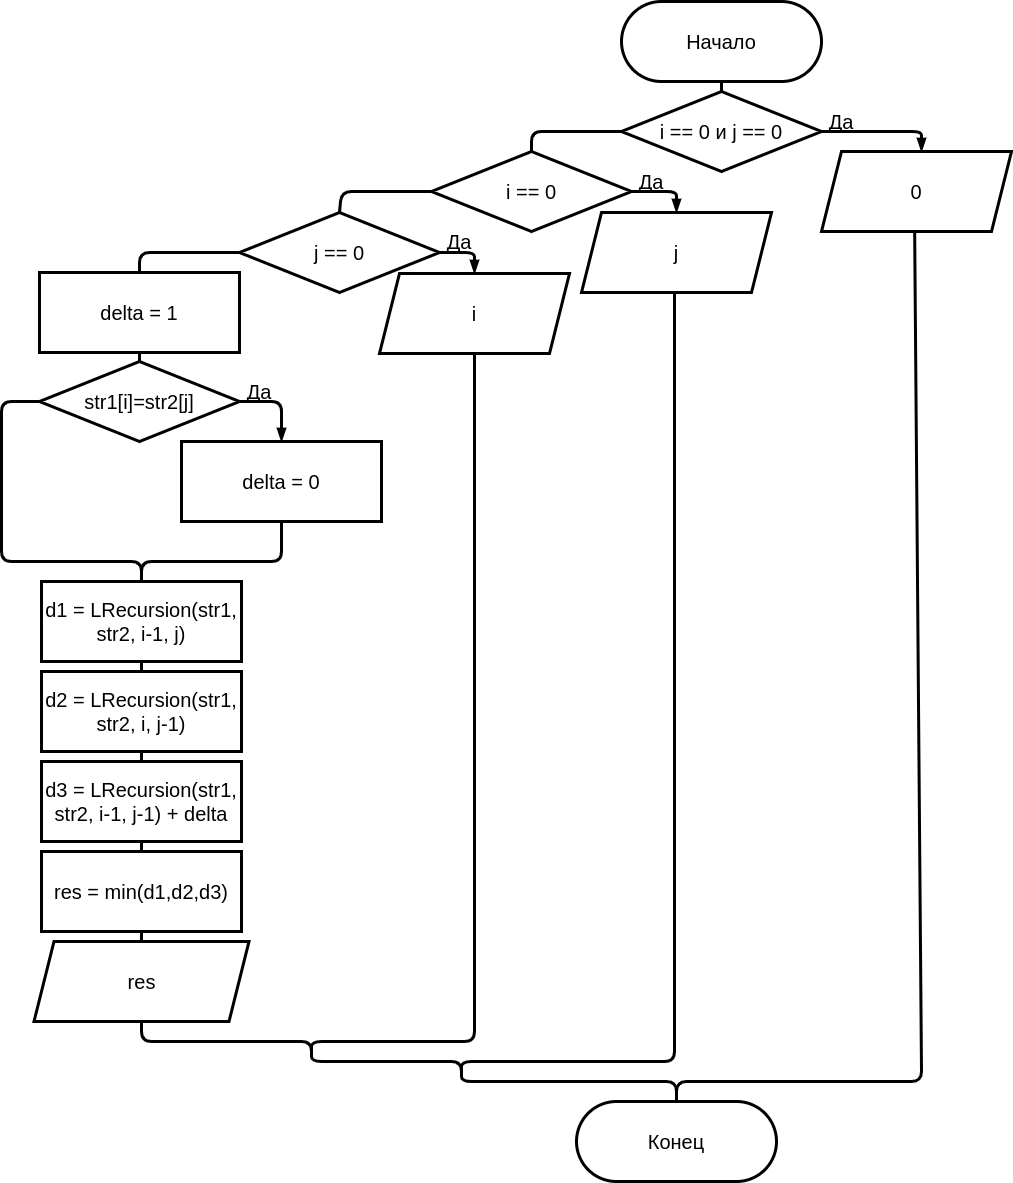
\includegraphics[scale=0.35]{l1.levenshteinrecursiveschema}}
    \caption{Схема алгоритма нахождения расстояния Левенштейна рекурсивным способом}
    \label{ris:levenshteinDamerayrecursiveschema}
\end{figure}

\section{Структуры данных}\label{Structs}

При реализации приведенных алгоритмов потребуются следующие типы данных: матрица, 
специализированная матрица для нахождения расстояния Левенштейна, ассоциативный массив.

\section{Тестирование}\label{Testing}

\subsection{Классы эквивалентности}\label{TestingClasses}

Для алгоритма Левенштейна можно выделить следующие классы эквивалентности:

\begin{enumerate}
    \item По длине строки
    \begin{enumerate}
        \item Строки одинаковой длины
        \item Строки разной длины
    \end{enumerate} 
    \item По количеству одинаковых символов
    \begin{enumerate}
        \item Одна строка входит в другую
        \item В строках есть повторяющиеся части
        \item В строках нет повторяющихся символов
    \end{enumerate} 
\end{enumerate}

Для алгоритма Дамерау-Левенштейна можно выделить следующие классы эквивалентности.

\begin{enumerate}
    \item По длине строки
    \begin{enumerate}
        \item Строки одинаковой длины
        \item Строки разной длины
    \end{enumerate} 
    \item По количеству одинаковых символов
    \begin{enumerate}
        \item Одна строка входит в другую
        \item В строках есть повторяющиеся части
        \item В строках нет повторяющихся символов
    \end{enumerate} 
    \item По наличию опечаток
    \begin{enumerate}
        \item В строке есть опечатка (пе->еп)
        \item В строке опчатки нет (пе->еп)
    \end{enumerate} 
\end{enumerate}


\subsection{Способы тестирования}\label{TestingMethods}

При разработке программы удобно использовать следующие методы тестирования:

\begin{enumerate}
    \item Модульные тесты 
    \item Функциональные тесты 
\end{enumerate} 

\section{Вывод конструкторской части}\label{KonstructResult}
На основе данных, полученных в аналитическом разделе, были построены схемы используемых алгоритмов,
выделены необходимые для реализации структуры данных и методы тестирования.

